\subsection{x86}

\subsubsection{MSVC}

\RU{Компилируем}\EN{Let's compile}:

\lstinputlisting[caption=MSVC 2008]{patterns/13_arrays/1_simple/simple_msvc.asm}

\index{x86!\Instructions!SHL}
\RU{Однако, ничего особенного, просто два цикла, один заполняет цикл, второй печатает его содержимое. 
Команда \TT{shl ecx, 1} используется для умножения \ECX на 2, об этом ниже~(\ref{SHR}).}
\EN{Nothing very special, just two loops: first is filling loop and second is printing loop.
\TT{shl ecx, 1} instruction is used for value multiplication by 2 in the \ECX, more about below~\ref{SHR}.}

\RU{Под массив выделено в стеке $80$ байт, это $20$ элементов по $4$ байта.}
\EN{$80$ bytes are allocated on the stack for array, that is $20$ elements of $4$ bytes.}

\RU{Попробуем этот пример в}\EN{Let's try this example in} \olly.
\index{\olly}

\RU{Видно как заполнился массив}\EN{We see how array gets filled}: 
\RU{каждый элемент это 32-битное слово типа \Tint, с шагом 2}
\EN{each element is 32-bit word of \Tint type, step by 2}: \figref{fig:array_simple_olly}.
\RU{А так как этот массив находится в стеке, то мы видим все его 20 элементов внутри стека}
\EN{Since this array is located in stack, we see all its 20 elements inside of stack}.

\begin{figure}[H]
\centering
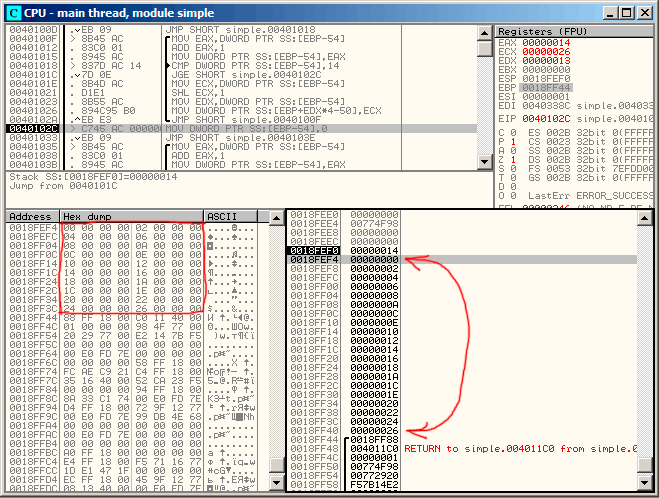
\includegraphics[scale=\FigScale]{patterns/13_arrays/1_simple/olly.png}
\caption{\olly: \RU{после заполнения массива}\EN{after array filling}}
\label{fig:array_simple_olly}
\end{figure}

\subsubsection{GCC}

\RU{То, что делает GCC 4.4.1:}\EN{Here is what GCC 4.4.1 does:}

\lstinputlisting[caption=GCC 4.4.1]{patterns/13_arrays/1_simple/simple_gcc.asm}

\RU{Кстати, переменная $a$ в нашем примере имеет тип \IT{int*} (то есть, указатель на \Tint{}) ~--- вы можете попробовать передать в другую функцию указатель на массив, но точнее было бы сказать, что передается указатель на первый элемент массива (а адреса остальных элементов массива можно вычислить очевидным образом).}\EN{By the way, $a$ variable has \IT{int*} type 
(the pointer to \Tint{})~---you can try to pass a pointer to array to another function, but it much correctly to say the pointer to the first array element is passed (addresses of another element's places are calculated in obvious way).}
\RU{Если индексировать этот указатель как \IT{a[idx]}, \IT{idx} просто прибавляется к указателю и возвращается элемент, расположенный там, куда ссылается вычисленный указатель.}\EN{If to index this pointer as \IT{a[idx]}, \IT{idx} just to be added to the pointer and the element placed there (to which calculated pointer is pointing) returned.}

\RU{Вот любопытный пример: строка символов вроде \IT{``string''} это массив из символов, 
и она имеет тип \IT{const char[]}.}\EN{An interesting example: string of characters like 
\IT{``string''} is array of characters and it has \IT{const char[]} type.}\RU{К этому указателю 
также можно применять индекc.}\EN{Index can be applied to this pointer.}
\RU{И поэтому можно написать даже так:  \TT{``string''[i]} ~--- это совершенно легальное выражение в \CCpp!}
\EN{And that is why it is possible to write like \TT{``string''[i]}~---this is correct \CCpp expression!}
